% Foliensatz: "AFu-Kurs nach DJ4UF" von DK0TU, Amateurfunkgruppe der TU Berlin
% Lizenz: CC BY-NC-SA 3.0 de (http://creativecommons.org/licenses/by-nc-sa/3.0/de/)
% Autoren: Martin Deutschmann <martin.deutschmann@campus.tu-berlin.de>

\documentclass[aspectratio=169]{beamer}

\usepackage[ngerman]{babel} % deutsche Worttrennung etc.
\usepackage[utf8]{inputenc} % UTF8 Text

\usepackage[super, comma, numbers, square, sort]{natbib}

\usepackage{hyperref}       % Hyperref Package für bessere Referenzen (todo)
\hypersetup{
	colorlinks=false,       %   false: boxed links; true: colored links
    %linkcolor=white,       %   color of internal links (change box color with linkbordercolor)
    citecolor=red,          %   color of links to bibliography
    filecolor=white,        %   color of file links
    urlcolor=blue           %   color of external links
}

\usepackage{multirow}
\usepackage{wasysym}  % Math Symbols like \permil
%\usepackage{colortbl}
%\usepackage{subscript}
%\usepackage{caption}
%\usepackage{setspace}
%\usepackage{xcolor}        % benutze CodeListe

% Footnote
%\usepackage{hanging}
%
%\setbeamertemplate{footnote}{%
%  \hangpara{2em}{1}%
%  \makebox[2em][l]{\insertfootnotemark}\footnotesize\insertfootnotetext\par%
%}


%\usepackage{pgf}
%\usepackage{tikz}
%\usetikzlibrary{arrows,automata}
%\usetikzlibrary{positioning}
%
%\tikzset{
%    state/.style={
%           rectangle,
%           rounded corners,
%           draw=black, very thick,
%           minimum height=2em,
%           minimum width=2pt,
%           inner sep=2pt,
%           text centered,
%           },
%}

%\usepackage{listings}
%\lstset{basicstyle=\small, numberstyle=\tiny, extendedchars=true, numbers=left, numbersep=5pt}
%\lstset{showtabs=false, showspaces=false, showstringspaces=false}
%%\lstset{backgroundcolor=\color{white!75!lightgray}, , frame=single}
%%\lstset{backgroundcolor=\color{white}}
%%\lstset{backgroundcolor=none}
%\lstset{keywordstyle=\color{blue!50!gray},  identifierstyle=\color{black}}
%\lstset{commentstyle=\color{green!50!gray}, stringstyle=\color{red!50!gray}}
%\lstset{language=C, fontadjust=true, tabsize=2, breaklines=true}
%\lstset{backgroundcolor=\color{white!75!lightgray}, caption=\lstname, frame=single}
%\lstset{emphstyle=\color{black}\fbox}
%
%% Keine "Listing:"-Caption
%\captionsetup{labelformat=empty,labelsep=none}
%
%% für mathematische Umgebungen
%\usepackage{amsmath,amsfonts,amssymb}
%
%\lstdefinestyle{Bash}{
%language=Bash,
%frame=single,
%rulecolor=\color{black},
%backgroundcolor=\color{gray!50},
%keywordstyle=\color{black},
%identifierstyle=,
%commentstyle=\color{black},
%stringstyle=\color{magenta!65!white},
%showstringspaces=false,
%basicstyle=\footnotesize\ttfamily\color{black},
%numbers=none,
%breaklines=true,
%captionpos=b
%}

%\usepackage{listings}
%
%\lstdefinestyle{basic}{
%    captionpos=t,%
%    basicstyle=\footnotesize\ttfamily,%
%    numberstyle=\tiny,%
%    numbers=left,%
%    stepnumber=1,%
%    frame=single,%
%    showspaces=false,%
%    showstringspaces=false,%
%    showtabs=false,%
%    %
%    keywordstyle=\color{blue},%
%    identifierstyle=,%
%    commentstyle=\color{gray},%
%    stringstyle=\color{magenta}%
%}



% fließende Boxen haben keinen Abstand
%\fboxsep0mm

% inkludiere Creative Commons Helper
%%%%%%%%%%%%%%%%%%%%%%%%%%%%%%%%%%%%%%%%%%%%%%%%%%%%%%%%%%%%%%%%
%% ccBeamer 0.1, 2007-07-02                                   %%
%% Written by Sebastian Pipping <webmaster@hartwork.org>      %%
%% ---------------------------------------------------------- %%
%% Licensed under Creative Commons Attribution-ShareAlike 3.0 %%
%% http://creativecommons.org/licenses/by-sa/3.0/             %%
%%%%%%%%%%%%%%%%%%%%%%%%%%%%%%%%%%%%%%%%%%%%%%%%%%%%%%%%%%%%%%%%


%% Images
\newcommand{\CcImageBy}[1]{%
	
\includegraphics[scale=#1]{texdata/creative_commons/cc_by_30.pdf}%
}
\newcommand{\CcImageCc}[1]{%
	
\includegraphics[scale=#1]{texdata/creative_commons/cc_cc_30.pdf}%
}
\newcommand{\CcImageDevNations}[1]{%
	
\includegraphics[scale=#1]{texdata/creative_commons/cc_dev_nations_30.pdf}%
}
\newcommand{\CcImageNc}[1]{%
	
\includegraphics[scale=#1]{texdata/creative_commons/cc_nc_30.pdf}%
}
\newcommand{\CcImageNd}[1]{%
	
\includegraphics[scale=#1]{texdata/creative_commons/cc_nd_30.pdf}%
}
\newcommand{\CcImagePd}[1]{%
	
\includegraphics[scale=#1]{texdata/creative_commons/cc_pd_30.pdf}%
}
\newcommand{\CcImageSa}[1]{%
	
\includegraphics[scale=#1]{texdata/creative_commons/cc_sa_30.pdf}%
}
\newcommand{\CcImageSampling}[1]{%
	
\includegraphics[scale=#1]{texdata/creative_commons/cc_sampling_30.pdf}%
}
\newcommand{\CcImageSamplingPlus}[1]{%
	
\includegraphics[scale=#1]{texdata/creative_commons/cc_sampling_plus_30.pdf}%
}


%% Groups
\newcommand{\CcGroupBy}[2]{% zoom, gap
	\CcImageCc{#1}\hspace*{#2}\CcImageBy{#1}%
}
\newcommand{\CcGroupByNc}[2]{% zoom, gap
	\CcImageCc{#1}\hspace*{#2}\CcImageBy{#1}\hspace*{#2}\CcImageNc{#1}%
}
\newcommand{\CcGroupByNcNd}[2]{% zoom, gap
	\CcImageCc{#1}\hspace*{#2}\CcImageBy{#1}\hspace*{#2}\CcImageNc{#1}\hspace*{#2}\CcImageNd{#1}%
}
\newcommand{\CcGroupByNcSa}[2]{% zoom, gap
	\CcImageCc{#1}\hspace*{#2}\CcImageBy{#1}\hspace*{#2}\CcImageNc{#1}\hspace*{#2}\CcImageSa{#1}%
}
\newcommand{\CcGroupByNd}[2]{% zoom, gap
	\CcImageCc{#1}\hspace*{#2}\CcImageBy{#1}\hspace*{#2}\CcImageNd{#1}%
}
\newcommand{\CcGroupBySa}[2]{% zoom, gap
	\CcImageCc{#1}\hspace*{#2}\CcImageBy{#1}\hspace*{#2}\CcImageSa{#1}%
}
\newcommand{\CcGroupDevNations}[2]{% zoom, gap
	\CcImageCc{#1}\hspace*{#2}\CcImageDevNations{#1}%
}
\newcommand{\CcGroupNcSampling}[2]{% zoom, gap
	\CcImageCc{#1}\hspace*{#2}\CcImageNc{#1}\hspace*{#2}\CcImageSampling{#1}%
}
\newcommand{\CcGroupPd}[1]{% zoom
	\CcImagePd{#1}%
}
\newcommand{\CcGroupSampling}[1]{% zoom
	\CcImageSampling{#1}%
}
\newcommand{\CcGroupSamplingPlus}[1]{% zoom
	\CcImageSamplingPlus{#1}%
}


%% Text
\newcommand{\CcLongnameBy}{Attribution}
\newcommand{\CcLongnameByNc}{Attribution-NonCommercial}
\newcommand{\CcLongnameByNcNd}{Attribution-NoDerivs}
\newcommand{\CcLongnameByNcSa}{Attribution-NonCommercial-ShareAlike}
\newcommand{\CcLongnameByNd}{Attribution-NoDerivs}
\newcommand{\CcLongnameBySa}{Attribution-ShareAlike}

\newcommand{\CcNote}[1]{% longname
	This work is licensed under the \textit{Creative Commons #1 3.0 License}.%
}


% generelles Thema auswählen
\usetheme{Goettingen} %Berlin spart ohne Sidebar allerdings angenehm Platz
% AnnArbor | Antibes | Bergen | Berkeley | Berlin | Boadilla | boxes | CambridgeUS | Copenhagen | Darmstadt | default | Dresden | Frankfurt | Goettingen | Hannover | Ilmenau | JuanLesPins | Luebeck | Madrid | Malmoe | Marburg | Montpellier | PaloAlto | Pittsburgh | Rochester | Singapore | Szeged | Warsaw

% Farben wählen
\usecolortheme{beetle}
% beaver | beetle | crane | default | dolphin | dove | fly | lily | orchid | rose | seagull | seahorse | sidebartab | structure | whale | wolverine

% Setze alle Farben auf Grau und Weiß
%\definecolor{craneorange}{RGB}{64,64,64}
%\definecolor{craneblue}{RGB}{255,255,255}

% Schriftart wählen
\usefonttheme{default}
% default | professionalfonts | serif | structurebold | structureitalicserif | structuresmallcapsserif

% Innere Themen(Kopf-, Fuß-, Sidebar usw)
%\useinnertheme{default}
\useinnertheme{circles}
% default | inmargin | rectangles | rounded | circles

% Äußere Themen (Anordnung der inneren, grenzen der Folien etc.)
\useoutertheme{infolines}
% default | infolines | miniframes | shadow | sidebar | smoothbars | smoothtree | split | tree

% Deaktiviere Navigations-Symbole ({} -> leer)
\setbeamertemplate{navigation symbols}{}
%\setbeamertemplate{navigation symbols}{\large \ifnum \insertframenumber <10 0\fi\insertframenumber/\inserttotalframenumber\vspace*{0.2ex}}

% Zeige ein Hintergrundbild
\setbeamertemplate{background canvas}{
        \hspace*{-2.0cm}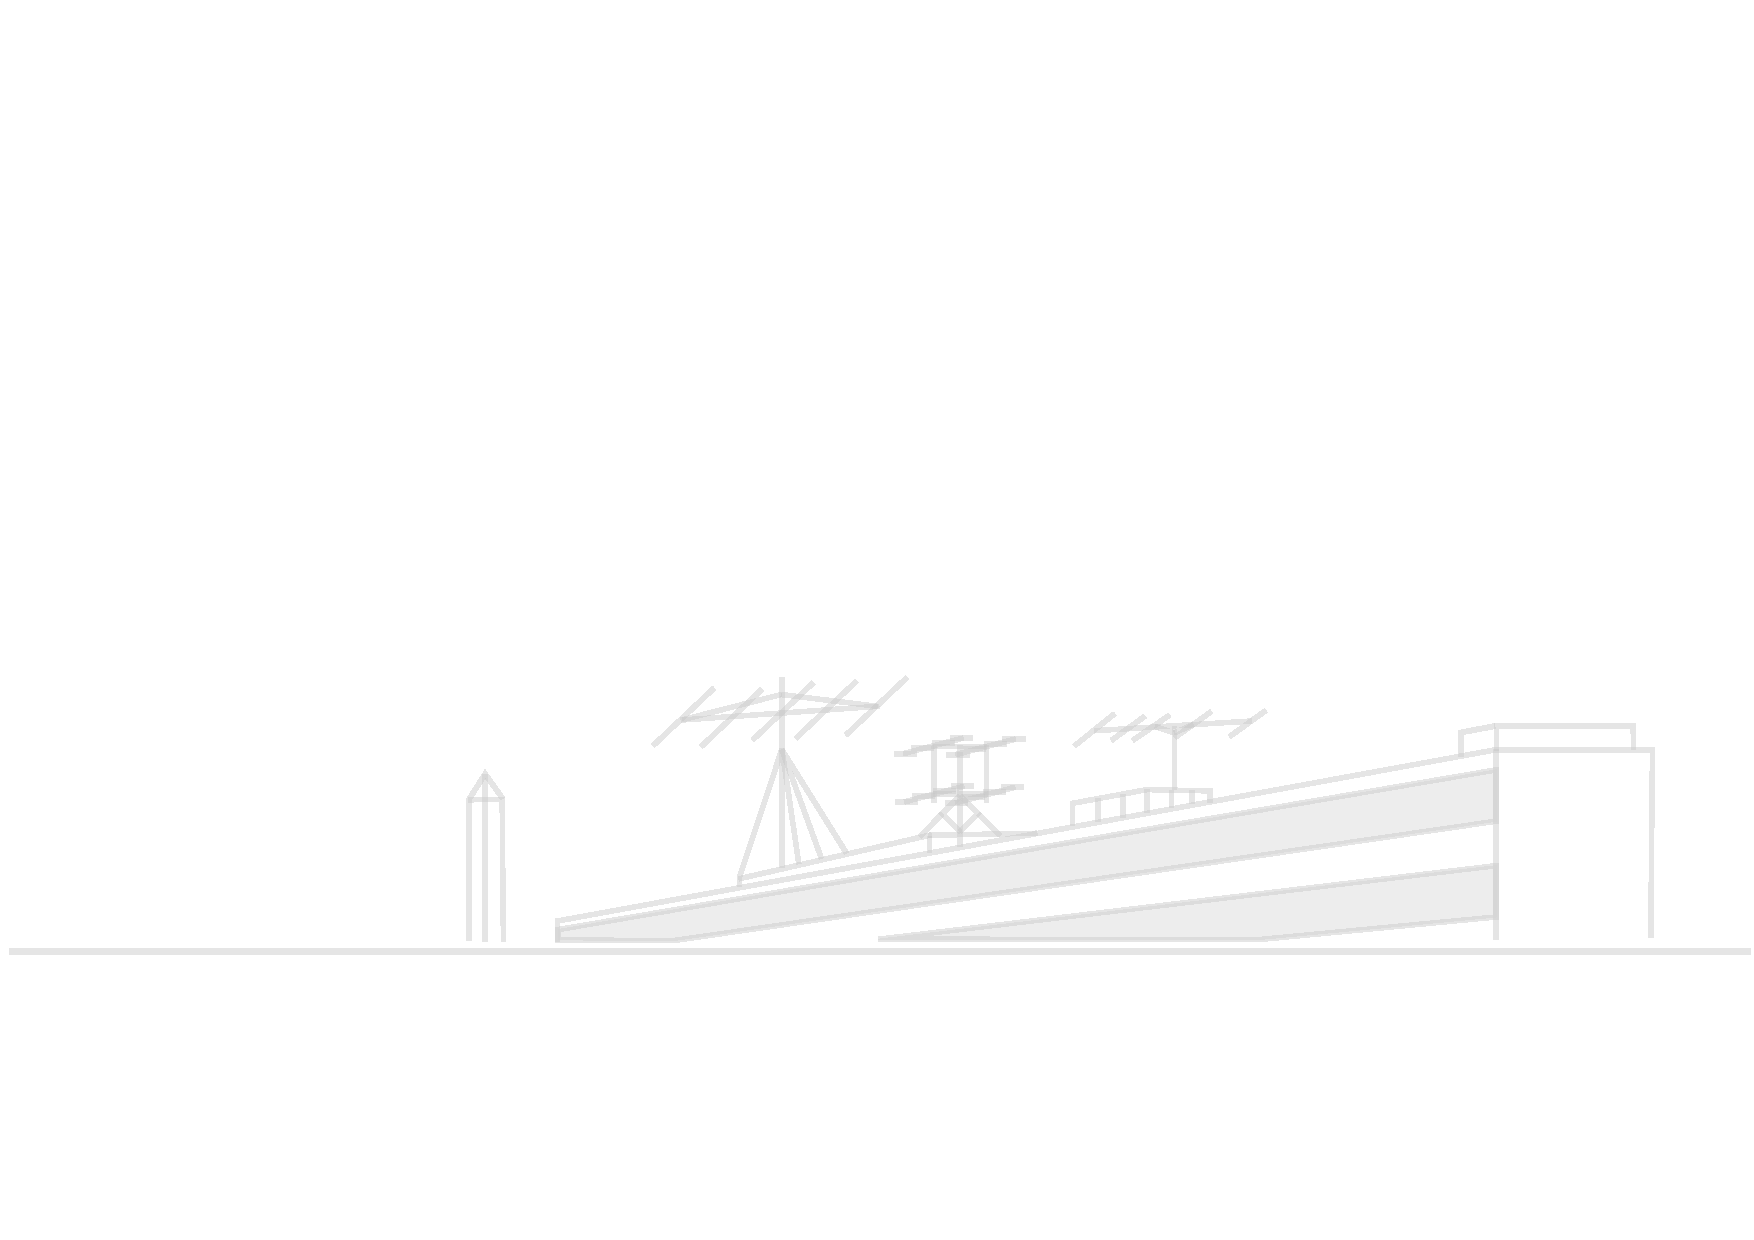
\includegraphics[width=17.8cm]{texdata/dk0tu_rooftop_background.pdf}
}

% Foliennummer einfügen
\setbeamertemplate{footline}[frame number]
%\setbeamertemplate{footline}{}

% Ändere das Zeichen vor jedem item
%\setbeamertemplate{itemize item}{\color{craneorange}$\blacktriangleright$}
%\setbeamertemplate{itemize subitem}{\color{craneorange}$\triangleright$}
%\setbeamertemplate{itemize subsubitem}{\color{craneorange}$\blacktriangleright$}

% Ändert die Blöcke 
\setbeamertemplate{blocks}[rounded][shadow=true]
% default | rounded [shadow=true|false]

%
% Eigene Kommandos
%

% Hack to get natbib and beamer working together. "The beamer user guide suggests
% that only the manual bibliography entry approach is supported"
% on some system it works out of the box, sometimes you need the hack :-(
% so check it --dl7bst
\ifdefined\newblock
    \relax
\else
    \newcommand{\newblock}{}
\fi

% \includedia command to generate png out of a dia file
% NEEDS installed dia and pdflatex option --shell-escape
\newcommand{\includedia}[1]{
    \immediate\write18{/usr/bin/dia #1.dia -e #1_diatmp.png -t png}
}

% RICHIG GROSSER FONT!
\newfont{\bigfont}{cmr10 at 144pt}
\newfont{\smallfont}{cmr10 at 8pt}

% Römische Ziffern
\makeatletter
\newcommand{\rmnum}[1]{\romannumeral #1}
\newcommand{\Rmnum}[1]{\expandafter\@slowromancap\romannumeral #1@}
\makeatother

% Schwarze Überschrift
%\setbeamercolor{frametitle}{fg=black}
%\setbeamercolor{title}{fg=black}

% Item- und Box-Farben
\definecolor{deepBlue}{HTML}{000066}
\setbeamercolor{itemize item}{fg=deepBlue}
\setbeamercolor{itemize subitem}{fg=deepBlue}
\setbeamercolor{description item}{fg=deepBlue}
\setbeamercolor{block title}{fg=deepBlue!100, bg=blue!15}
\setbeamercolor{block body}{fg=black, bg=blue!5}
\setbeamercolor{block title alerted}{fg=deepBlue, bg=red!75}
\setbeamercolor{block body alerted}{fg=black, bg=red!15}
\setbeamercolor*{block title example}{fg=blue!50, bg=blue!10}
\setbeamercolor*{block body example}{fg= blue, bg=blue!5}

%\setbeamercolor{section in head/foot}{parent=palette primary}
%\setbeamercolor{subsection in head/foot}{parent=palette secondary}
%\setbeamercolor{sidebar}{fg=darkblue,bg=yellow!90!orange}
%\setbeamercolor{title in sidebar}{fg=darkblue}
%\setbeamercolor{author in sidebar}{fg=darkblue}
%\setbeamercolor{section in sidebar}{fg=darkblue!10!black}
%\setbeamercolor{subsection in sidebar}{fg=darkblue!50!black}

% Titlepage Infos
\title{AFu-Kurs nach DJ4UF}
\author[DKØTU]{DKØTU\\ \footnotesize{Amateurfunkgruppe der TU Berlin}}
\institute[DKØTU]{\url{http://www.dk0tu.de} }

% PDF-Eigenschaften
\subject{DK0TU-Amateurfunkkurs nach DJ4UF}
\keywords{Amateurfunk Kurs HAM Radio Course CC-BY-NC-SA OpenSource TU Berlin DK0TU}

\subtitle{Technik Klasse E 03 \\
          Ohmsches Gesetz, Leistung \& Arbeit \\[2em]}
\date{Stand 30.10.2014}
 \begin{document}

\begin{frame}
    \titlepage
    \vfill
    \begin{center}
        \ccbyncsaeu\\
        {\tiny This work is licensed under the \em{Creative Commons Attribution-NonCommercial-ShareAlike 3.0 License}.}\\[0.5ex]
         \tiny Amateurfunkgruppe der Technische Universität Berlin (AfuTUB), DKØTU
         %\includegraphics[scale=0.5]{img/DK0TU_Logo.pdf}
    \end{center}
\end{frame}


%fixme Referenzen, Link funktioniert auch nicht

\section{das ohmsche Gesetz}

\begin{frame}
    \frametitle{Was ist das ohmsche Gesetz?}
    \begin{itemize}
    	\item Das ohmsche Gesetz ist folgendes:
    \end{itemize}
    \begin{center}
 		
\includegraphics[scale=0.3]{e03/Ohm_law_triangle.png}
 		\footnote{Abb.1: das ohmsche Dreieck \cite{wmen}}
 	\end{center}
 	\begin{itemize}
 		\item	Aber was sagt uns das nun?
 	\end{itemize}
\end{frame}

\begin{frame}
	\frametitle{Das ohmsche Gesetz}
	\begin{itemize}
		\item	Das ohmsche Gesetz gibt uns die Abhängigkeiten zwischen Spannung, Strom \& ohmschen Widerstand an
		\item	Dadurch wissen wir, das sich zum Beispiel der Strom an einem konstanten Widerstand proportional zur Spannung ändert
	\end{itemize}
\end{frame}

\begin{frame}
	\frametitle{Ein kleines Gedankenexperiment}
	\begin{itemize}
		\item	Wir stellen uns folgenden Aufbau vor:
		\item	Der Widerstand der Lampe soll 1 $\Omega$ betragen
	\end{itemize}
	\begin{center}
 		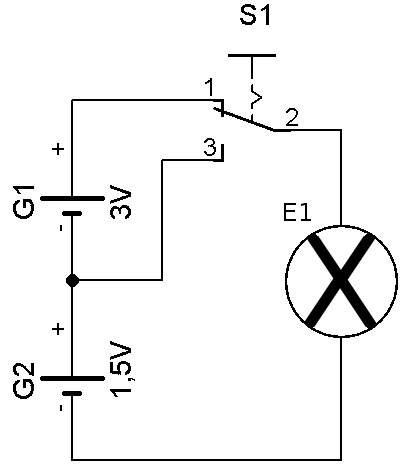
\includegraphics[scale=1]{e03/Strom_Spannung_Abh.png}
 		\footnote{Abb.2: Helligkeit einer Lampe bei verschiedenen Spannungen}
 	\end{center}
 	\begin{itemize}
 		\item	Wird die Lampe heller oder dunkler, wenn man sie mit 1,5 Volt anstatt mit 4,5 Volt betreibt?
 	\end{itemize}
\end{frame}

\begin{frame}
	\frametitle{wie funktioniert das Ohmsche Dreieck}
	\begin{itemize}
		\item	Nun wollen wir wissen, wie viel Strom in beiden Fällen unseres Gedankenexperimentes fließt
		\item	Dazu nehmen wir uns das Ohmsche Dreieck zu Hilfe
	\end{itemize}
	\begin{center}
 		
\includegraphics[scale=0.2]{e03/Ohm_law_triangle.png}
 		\footnote{Abb.3: das ohmsche Dreieck \cite{wmen}}
 	\end{center}
 	\begin{itemize}
 		\item	Decken wir den Wert, den wir ermitteln wollen ab, so zeigt uns das Dreieck die Formel dafür
 		\item	So lautet die Formel für den Strom:
 	\end{itemize}
 	\begin{equation}
 		I = \frac{U}{R}
 		\label{equ:Strom}
 	\end{equation}
\end{frame}

\begin{frame}
	\frametitle{Das Ergebnis unseres Experimentes}
	\begin{itemize}
		\item	Setzen wir nun die Werte in diese Formel ein, so erhalten wir
	\end{itemize}
	\begin{equation}
		I_{4,5 V} = \frac{4,5 V}{1 \Omega} = 4,5 A
	\end{equation}
	\begin{itemize}
		\item Sowie
	\end{itemize}
	\begin{equation}
		I_{1,5 V} = \frac{1,5 V}{1 \Omega} = 1,5 A
	\end{equation}
	\begin{itemize}
		\item	Womit bei 4,5 Volt angelegter Spannung der größere Strom durch die Lampe fließt
	\end{itemize}
\end{frame}

\begin{frame}
	\frametitle{Der Innenwiderstand}
	\begin{itemize}
		\item	Oftmals bemerken wir einen Spannungsabfall, zwischen einer Maschine im Leerlauf und der gleichen Maschine bei Belastung
		\item	Dies führen wir auf den Innenwiderstand der Maschine zurück
	\end{itemize}
	\begin{center}
 		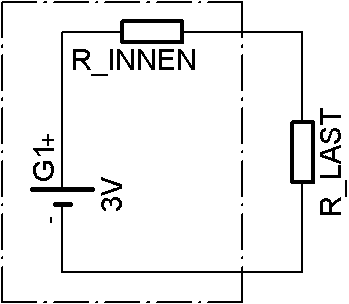
\includegraphics[scale=1.4]{e03/Innenwiderstand.png}
 		\footnote{Abb.4: Innenwidestand einer Batterie}
 	\end{center}
\end{frame}

\begin{frame}
	\frametitle{der Innenwiderstand}
	\begin{itemize}
		\item	Um den Innenwiderstand zu ermitteln nutzen wir wieder das ohmsche Gesetz
		\item	Dabei gilt es zu beachten, das diesmal die Differenzen der Spannungen und des Stromes zwischen dem Leerlauf und dem belasteten Fall verrechnet werden
		\item	Es gilt:
	\end{itemize}
	\begin{equation}
		R_{innen} = \frac{\Delta U}{\Delta I}
	\end{equation}
	\begin{itemize}
		\item	Um den Wert nicht zu sehr zu verfälschen sollten Spannungsquellen einen niedrigen und Stromquellen einen hohen Innenwiderstand besitzen
	\end{itemize}
\end{frame}

\begin{frame}
	\begin{small}	
	\begin{tabular}{|l|l|l|}
	\hline
		\multicolumn{3}{|c|}{\textbf{TD302:} Die Leerlaufspannung einer Gleichspannungsquelle}\\
		\multicolumn{3}{|c|}{beträgt 13,5 V. Wenn die Spannungsquelle einen Strom von 1 A}\\
		\multicolumn{3}{|c|}{abgibt, sinkt die Klemmenspannung auf 12,4 V. Wie groß ist der}\\			\multicolumn{3}{|c|}{Innenwiderstand der Spannungsquelle?}\\
		\hline
		A & $1,1 \Omega$ & ??? \\ \hline
		B & $1,2 \Omega$ & ??? \\ \hline
		C & $12,4 \Omega$ & ??? \\ \hline
		D & $13,5 \Omega$ & ??? \\ \hline 		
	\end{tabular}
	\end{small}
\end{frame}

\begin{frame}
	\begin{small}	
	\begin{tabular}{|l|l|l|}
	\hline
		\multicolumn{3}{|c|}{\textbf{TD302:} Die Leerlaufspannung einer Gleichspannungsquelle}\\
		\multicolumn{3}{|c|}{beträgt 13,5 V. Wenn die Spannungsquelle einen Strom von 1 A}\\
		\multicolumn{3}{|c|}{abgibt, sinkt die Klemmenspannung auf 12,4 V. Wie groß ist der}\\			\multicolumn{3}{|c|}{Innenwiderstand der Spannungsquelle?}\\
		\hline
		A & $1,1 \Omega$ & richtig \\ \hline
		B & $1,2 \Omega$ & ??? \\ \hline
		C & $12,4 \Omega$ & ??? \\ \hline
		D & $13,5 \Omega$ & ??? \\ \hline 		
	\end{tabular}
	\end{small}
	\vspace{1cm}
	\begin{equation}
		R = \frac{\Delta U}{\Delta I} = \frac{13,5V - 12,4V}{1A} = \frac{1,1V}{1A} = 1,1\Omega
	\end{equation}
\end{frame}

\begin{frame}
	\begin{small}	
	\begin{tabular}{|l|l|l|}
	\hline
		\multicolumn{3}{|c|}{\textbf{TD301:} Welche Eigenschaften sollten Strom- und}\\
		\multicolumn{3}{|c|}{Spannungsquellen aufweisen?}\\
		\hline
		A &  Strom- und Spannungsquellen sollten einen möglichst  & ??? \\
		" " & niedrigen Innenwiderstand haben. & " "\\ \hline
		B &  Strom- und Spannungsquellen sollten einen möglichst  & ??? \\
		" " & hohen Innenwiderstand haben. & " "\\ \hline
		C & Spannungsquellen sollten einen möglichst hohen & ??? \\
		" " & Innenwiderstand und Stromquellen einen möglichst  & " " \\ 
		" " & niedrigen Innenwiderstand haben.  & "" \\ \hline
		D & Spannungsquellen sollten einen möglichst niedrigen & ??? \\
		" " & Innenwiderstand und Stromquellen einen möglichst & " " \\ 
		" " & hohen Innenwiderstand haben.  & " " \\ \hline 		
	\end{tabular}
	\end{small}
\end{frame}

\begin{frame}
	\begin{small}	
	\begin{tabular}{|l|l|l|}
	\hline
		\multicolumn{3}{|c|}{\textbf{TD301:} Welche Eigenschaften sollten Strom- und}\\
		\multicolumn{3}{|c|}{Spannungsquellen aufweisen?}\\
		\hline
		A &  Strom- und Spannungsquellen sollten einen möglichst  & ??? \\
		" " & niedrigen Innenwiderstand haben. & " "\\ \hline
		B &  Strom- und Spannungsquellen sollten einen möglichst  & ??? \\
		" " & hohen Innenwiderstand haben. & " "\\ \hline
		C & Spannungsquellen sollten einen möglichst hohen & ??? \\
		" " & Innenwiderstand und Stromquellen einen möglichst  & " " \\ 
		" " & niedrigen Innenwiderstand haben.  & "" \\ \hline
		D & Spannungsquellen sollten einen möglichst niedrigen & richtig \\
		" " & Innenwiderstand und Stromquellen einen möglichst & " " \\ 
		" " & hohen Innenwiderstand haben.  & " " \\ \hline 		
	\end{tabular}
	\end{small}
\end{frame}

\section{die elektrische Leistung}
\begin{frame}
	\frametitle{die elektrische Leistung}
	\begin{itemize}
		\item	Fließt ein Strom durch einen Widerstand, so entsteht Verlustleistung in Form von Wärme an dem Widerstand
		\item	Dies findet Anwendung bei Heizspiralen in Elektroherd, oder im Bügeleisen
		\item	In einer elektronischen Schaltung sollte diese Wärmeleistung aber so gering wie möglich sein
		\item	Um die Leistung zu ermitteln nutzen wir folgende Formel:
	\end{itemize}
	\begin{equation}
		P = U \cdot I
	\end{equation}
	\begin{itemize}
		\item	Die Einheit der Leistung ist das Watt
	\end{itemize}
	\begin{equation}
		 1[W] = 1[V] \cdot 1[A]
	\end{equation}
\end{frame}

\begin{frame}
	\begin{small}	
	\begin{tabular}{|l|l|l|}
	\hline
		\multicolumn{3}{|c|}{\textbf{TB906:} Eine Glühlampe hat einen Nennwert von 12 V }\\
		\multicolumn{3}{|c|}{und 48 W. Bei einer 12-V-Versorgung beträgt die Stromentnahme}\\
		\hline
		A & $36 A $ & ??? \\ \hline
		B & $250 mA $ & ??? \\ \hline
		C & $750 mA $ & ??? \\ \hline
		D & $4 A $ & ??? \\ \hline	
	\end{tabular}
	\end{small}
\end{frame}

\begin{frame}
	\begin{small}	
	\begin{tabular}{|l|l|l|}
	\hline
		\multicolumn{3}{|c|}{\textbf{TB906:} Eine Glühlampe hat einen Nennwert von 12 V }\\
		\multicolumn{3}{|c|}{und 48 W. Bei einer 12-V-Versorgung beträgt die Stromentnahme}\\
		\hline
		A & $36 A $ & ??? \\ \hline
		B & $250 mA $ & ??? \\ \hline
		C & $750 mA $ & ??? \\ \hline
		D & $4 A $ & richtig \\ \hline	
	\end{tabular}
	\end{small}
	\vspace{1cm}
	\begin{equation}
		I = \frac{P}{U} = \frac{48W}{12V} = 4A
	\end{equation}
\end{frame}

\section{die elektrische Arbeit}

\begin{frame}
	\frametitle{die elektrische Arbeit}
	\begin{itemize}
		\item	Die elektrische Arbeit ist definiert als die Leistung, die in einer bestimmten Zeit erbracht wurde
		\item	Es gilt also:
	\end{itemize}
	\begin{equation}
		W = P \cdot t
	\end{equation}
	\begin{itemize}
		\item	Wir können die Leistung auch als das Produkt von Strom und Spannung aufschreiben und erhalten dann:
	\end{itemize}
	\begin{equation}
		W = U \cdot I \cdot t
	\end{equation}
	\begin{itemize}
		\item	Die Einheit der elektrischen Arbeit ist die Wattsekunde [WS]
	\end{itemize}
\end{frame}

\begin{frame}
	\begin{small}	
	\begin{tabular}{|l|l|l|}
	\hline
		\multicolumn{3}{|c|}{\textbf{TB905:} Eine Stromversorgung nimmt bei 230 Volt einen Strom }\\
		\multicolumn{3}{|c|}{von 0,63 Ampere auf. Welche elektrische Arbeit  wird }\\
		\multicolumn{3}{|c|}{bei einer Betriebsdauer von 7 Stunden verbraucht?}\\
		\hline
		A & $1,01 kWh$ & ??? \\ \hline
		B & $0,1 kWh $ & ??? \\ \hline
		C & $2,56 kWh$ & ??? \\ \hline
		D & $20,7 kWh$ & ??? \\ \hline	
	\end{tabular}
	\end{small}
\end{frame}

\begin{frame}
	\begin{small}	
	\begin{tabular}{|l|l|l|}
	\hline
		\multicolumn{3}{|c|}{\textbf{TB905:} Eine Stromversorgung nimmt bei 230 Volt einen Strom }\\
		\multicolumn{3}{|c|}{von 0,63 Ampere auf. Welche elektrische Arbeit  wird }\\
		\multicolumn{3}{|c|}{bei einer Betriebsdauer von 7 Stunden verbraucht?}\\
		\hline
		A & $1,01 kWh$ & richtig \\ \hline
		B & $0,1 kWh $ & ??? \\ \hline
		C & $2,56 kWh$ & ??? \\ \hline
		D & $20,7 kWh$ & ??? \\ \hline	
	\end{tabular}
	\end{small}
	\vspace{1cm}
	\begin{equation}
		W = P \cdot t = U \cdot I \cdot t = 230V \cdot 0,63A \cdot 7h = 1,01kWh
	\end{equation}
\end{frame}

\renewcommand{\refname}{Referenzen}

\hypertarget{refs}{}
\textcolor{white}{} \\ %\vspace{} geht nicht
\Large Referenzen/Links
\footnotesize

\begin{thebibliography}{}
    \bibitem{e03}   Moltrecht E 03: \\
                    \url{http://www.darc.de/referate/ajw/ausbildung/darc-online-lehrgang/technik-klasse-e/technik-e03/}
    \bibitem{wp}    Wikipedia DE: \\
                    \url{http://de.wikipedia.org/wiki/Ohmsches_Gesetz}\\ 
                    \url{http://de.wikipedia.org/wiki/Elektrische_Leistung}\\ 
                    \url{http://de.wikipedia.org/wiki/lektrische_Energie#Elektrische_Energie_in_einem_elektrischen_Feld}\\ 
    \bibitem{wmde}	Wikimedia DE:\\
    				\url{http://commons.wikimedia.org/wiki/File:Ohmsches_Gesetz.svg?uselang=de}\\
   	\bibitem{wmen}	Wikimedia EN:\\
   					\url{http://commons.wikimedia.org/wiki/File:Ohm\%27s_law_triangle.PNG}\\
\end{thebibliography} 

% Hier könnte noch eine Kontaktfolie stehen

\end{document}

